
\section{Modelo de información del Plan de acción}

\subsection{Descripción general}
 En la figura~\ref{fig:planDeAccion} se muestra la estructura de información que manejará el sistema para registrar la información del plan de acción.
 
\begin{figure}[htbp!]
	\begin{center}
		\fbox{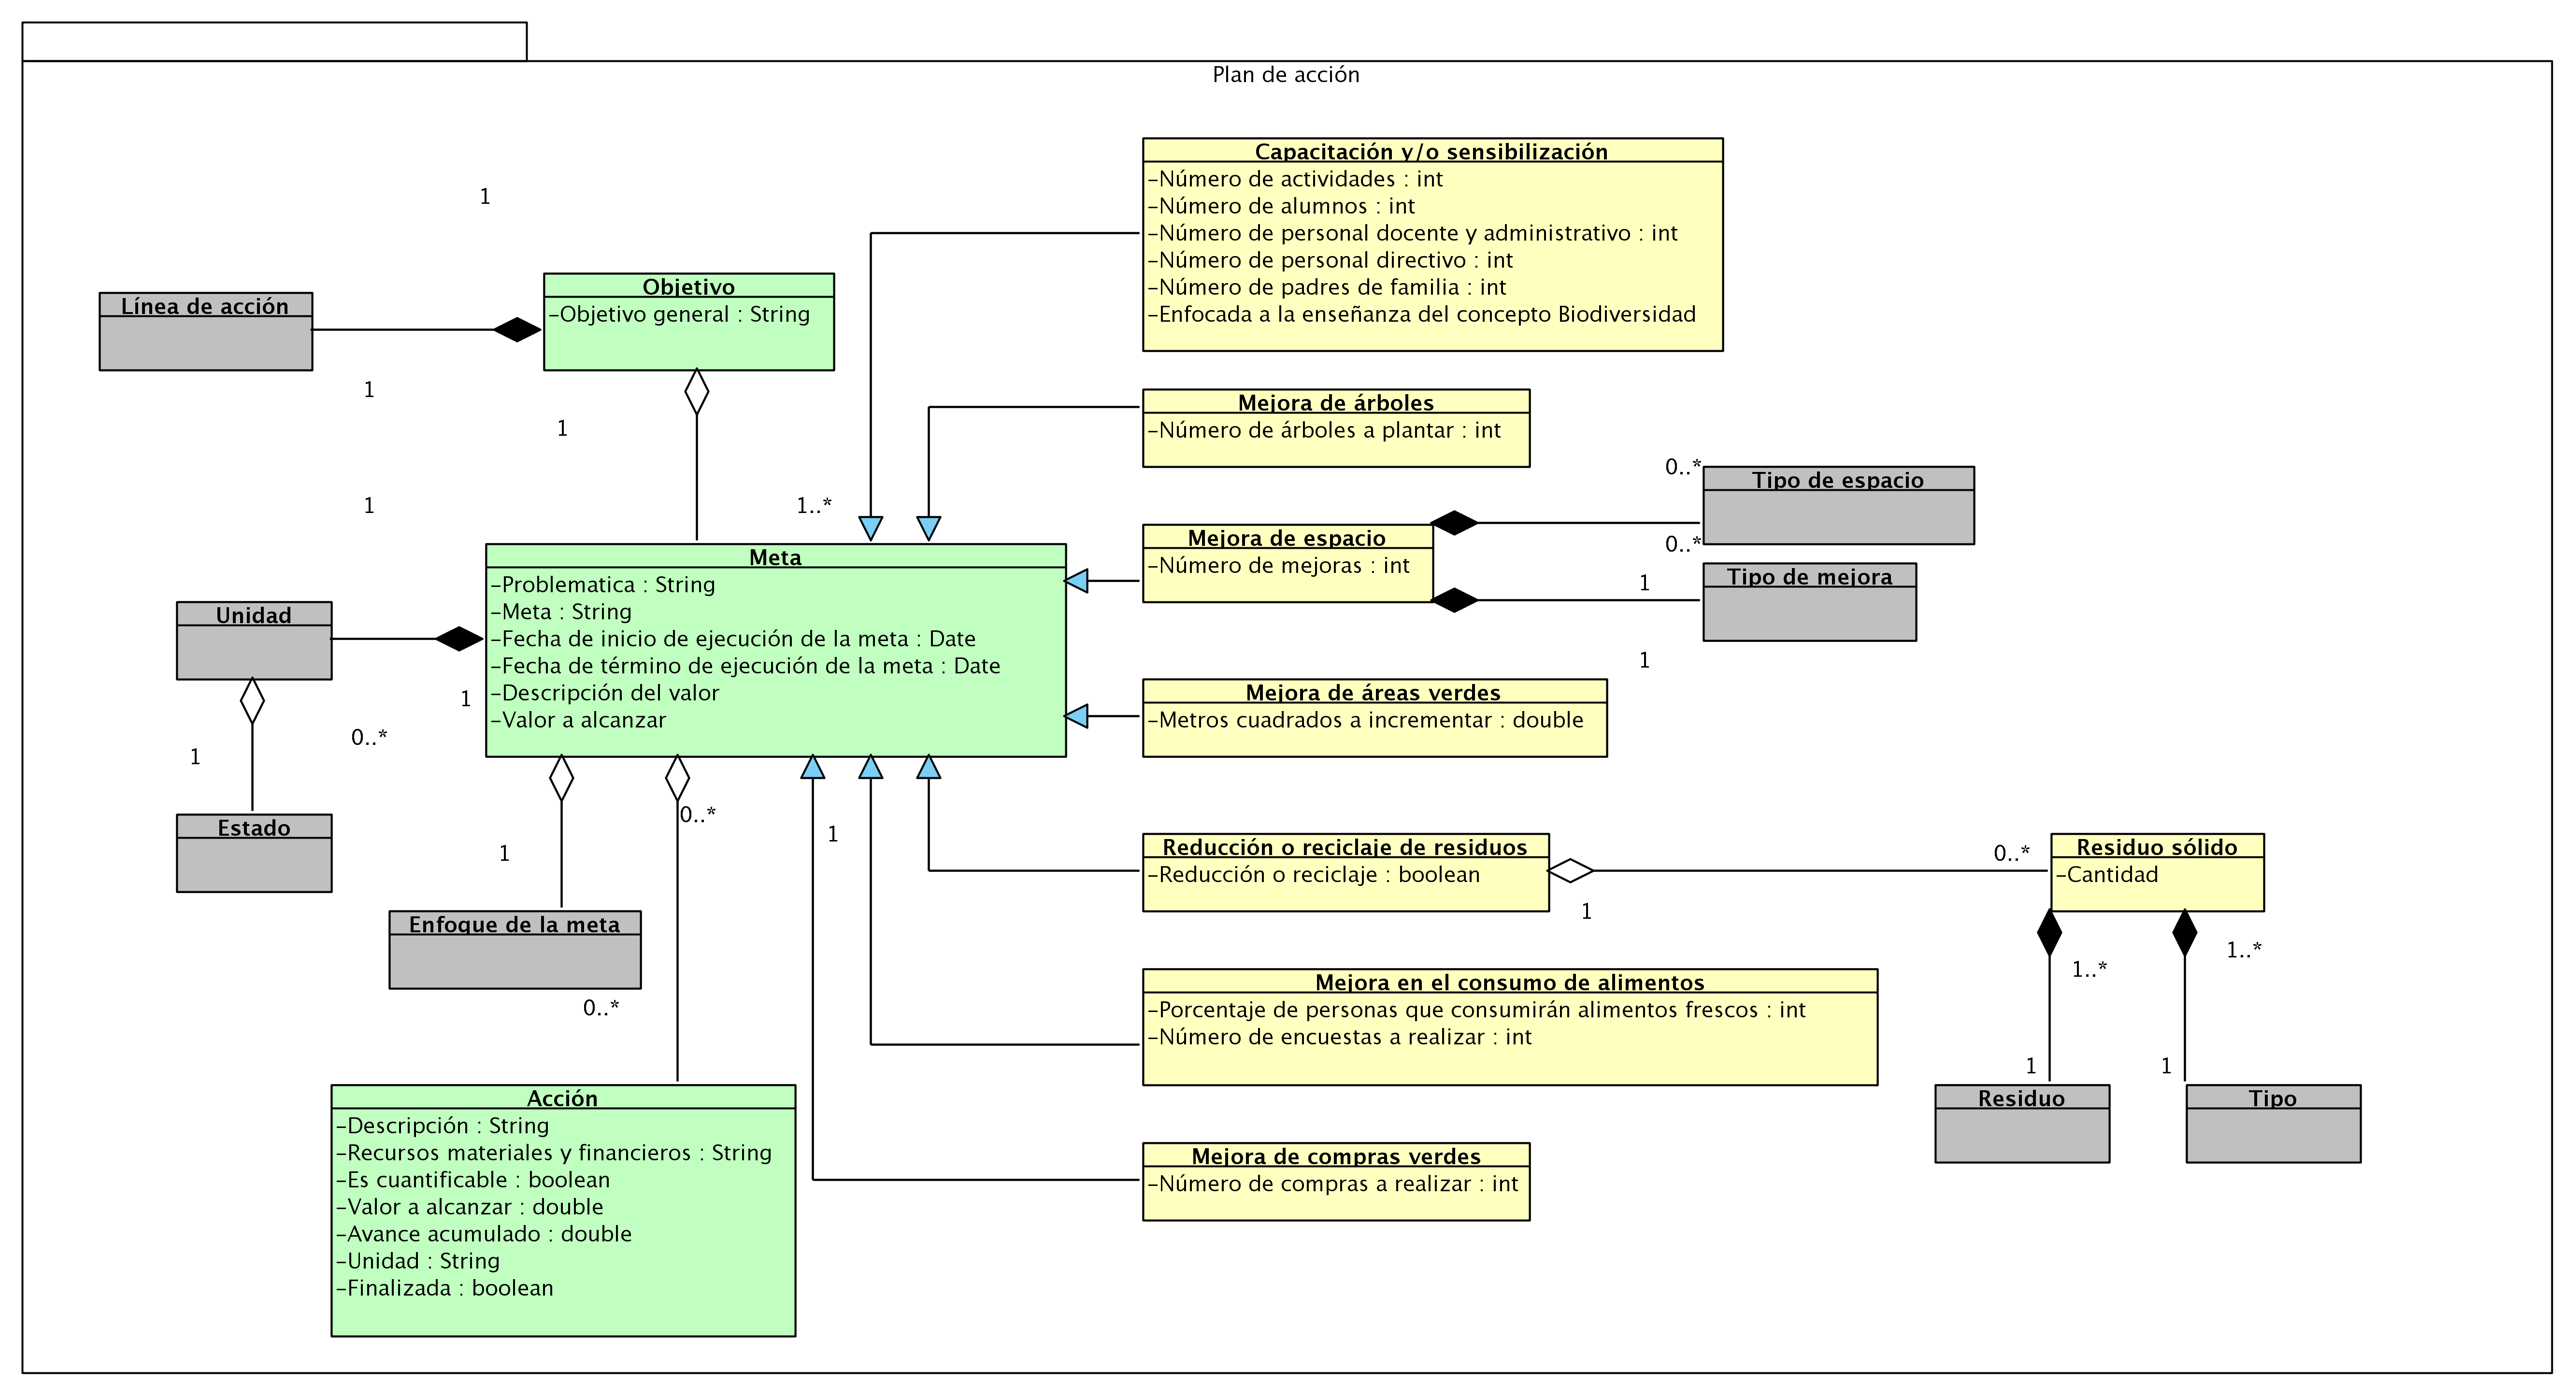
\includegraphics[width=1\textwidth]{images/clases/plan-accion}}
		\caption{Modelo de información del plan de acción.}
		\label{fig:planDeAccion}
	\end{center}
\end{figure}


\begin{BusinessEntity}{meta}{Meta}
      \Battr{problematica}{Problemática}{\tdParrafo}{Conjunto de problemas que serán atacados mediante el desarrollo de la meta}{\requerido}
      \Battr{meta}{Meta}{\tdParrafo}{Descripción del fin al que se dirigen las acciones}{\requerido}
      \Battr{fechaInicio}{Fecha de inicio de ejecución de la meta}{\tdFecha}{Fecha en la que se planea inicien las acciones para alcanzar la meta}{\requerido}
      \Battr{fechaTermino}{Fecha de término de ejecución de la meta}{\tdFecha}{Fecha en la que se planea terminen las acciones para alcanzar la meta}{\requerido}
      \Battr{nombreValor}{Descripción del valor a alcanzar}{\tdFrase}{Descripción de la característica cuantificable que va a ser medida para seguir el avance de una meta}{\requerido}
      \Battr{valorAlcanzar}{Valor a alcanzar}{\tdNumerico{entero}}{Valor que se establece como meta en el desarrollo del plan de acción}{\requerido}
      \Battr{enfoqueMeta}{Enfoque de la meta}{\tdCatalogo}{Fin al que se dirige una meta, definido por el catálogo \cdtRef{gls:enfoqueMeta}{Enfoque de la meta}}{\requerido}
\end{BusinessEntity}

\subsection{Relaciones}

\begin{BusinessFact}{meta:objetivo}{Objetivo}
      \BRitem{Descripción}{Un Objetivo cuenta con una o varias \cdtRef{meta}{Metas}}
      \BRitem{Tipo}{\relAsociacion}
      \BRitem{Cardinalidad}{Uno a muchos}
\end{BusinessFact}

\begin{BusinessFact}{meta:accion}{Acción}
      \BRitem{Descripción}{Una Meta cuenta con \cdtRef{accion}{Acciones}}
      \BRitem{Tipo}{\relAsociacion}
      \BRitem{Cardinalidad}{Uno a muchos}
\end{BusinessFact}

\begin{BusinessFact}{meta:capacitacionSensibilizacion}{Capacitación y/o sensibilización}
      \BRitem{Descripción}{Una Capacitación y/o sensibilización es un tipo de \cdtRef{meta}{Meta}}
      \BRitem{Tipo}{\relHerencia}
\end{BusinessFact}

\begin{BusinessFact}{meta:mejoraAraboles}{Mejora de árboles}
      \BRitem{Descripción}{Una Mejora de árboles es un tipo de \cdtRef{meta}{Meta}}
      \BRitem{Tipo}{\relHerencia}
\end{BusinessFact}

\begin{BusinessFact}{meta:mejoraEspacio}{Mejora de espacio}
      \BRitem{Descripción}{Una Mejora de espacio es un tipo de \cdtRef{meta}{Meta}}
      \BRitem{Tipo}{\relHerencia}
\end{BusinessFact}

\begin{BusinessFact}{meta:mejoraAreasVerdes}{Mejora de áreas verdes}
      \BRitem{Descripción}{Una Mejora de áreas verdes es un tipo de \cdtRef{meta}{Meta}}
      \BRitem{Tipo}{\relHerencia}
\end{BusinessFact}

\begin{BusinessFact}{meta:reduccionReciclaje}{Reducción o reciclaje de residuos}
      \BRitem{Descripción}{Una Reducción o reciclaje de residuos es un tipo de \cdtRef{meta}{Meta}}
      \BRitem{Tipo}{\relHerencia}
\end{BusinessFact}

\begin{BusinessFact}{meta:mejoraConsumoAlimentos}{Mejora en el consumo de alimentos}
      \BRitem{Descripción}{Una Mejora en el consumo de alimentos es un tipo de \cdtRef{meta}{Meta}}
      \BRitem{Tipo}{\relHerencia}
\end{BusinessFact}

\begin{BusinessFact}{meta:mejoraCompraVerdes}{Mejora de compras verdes}
      \BRitem{Descripción}{Una Mejora de compras verdes es un tipo de \cdtRef{meta}{Meta}}
      \BRitem{Tipo}{\relHerencia}
\end{BusinessFact}

\begin{BusinessFact}{meta:unidad}{Unidad}
      \BRitem{Descripción}{Una Meta cuenta con una o varias \cdtRef{unidad}{Unidades}}
      \BRitem{Tipo}{\relAsociacion}
      \BRitem{Cardinalidad}{Uno a muchos}
\end{BusinessFact}

%-----------------------------------------------------------------------------
\begin{BusinessEntity}{objetivo}{Objetivo}
      \Battr{objetivoGeneral}{Objetivo general}{\tdParrafo}{Fin o intento a que se dirige o encaminan las metas y acciones planteadas}{\requerido}
      \Battr{lineaAccion}{Línea de acción}{\tdCatalogo}{Orientación y organización de diferentes actividades relacionadas con los objetivos, definido por el catálogo \cdtRef{gls:lineaAccion}{Línea de acción}}{\requerido}
\end{BusinessEntity}

%-----------------------------------------------------------------------------
\begin{BusinessEntity}{unidad}{Unidad}
      \Battr{unidad}{Unidad}{\tdFrase}{Término que sirve como referencia para la medición de un valor}{\requerido}
      \Battr{estadoUnidad}{Estado}{\tdCatalogo}{Estado en el que se encuentra la unidad de medida, definido por el catálogo \cdtRef{gls:estadoUnidad}{Estado de la unidad} }{\requerido}
\end{BusinessEntity}

%----------------------------------------

\begin{BusinessEntity}{capacitacionSensibilizacion}{Capacitación y/o sensibilización}
      \Battr{numActividades}{Número de actividades}{\tdNumerico{entero}}{Cantidad de actividades que se planea realizar en la meta de capacitación y sensibilización}{\requerido}
      \Battr{numAlumnos}{Número de alumnos}{\tdNumerico{entero}}{Cantidad de alumnos que se planea asistan a la capacitación}{\requerido}
      \Battr{numDocenteAdministrativo}{Número de personal docente y administrativo}{\tdNumerico{entero}}{Cantidad de personal docente y administrativo que se planea asistan a la capacitación}{\requerido}
      \Battr{numDirectivos}{Número de personal directivo}{\tdNumerico{entero}}{Cantidad de personal directivo que se planea asistan a la capacitación}{\requerido}
      \Battr{numPadres}{Número de padres de familia}{\tdNumerico{entero}}{Cantidad de padres de familia que se planea asistan a la capacitación}{\requerido}
      \Battr{conceptoBiodiversidad}{Enfocada a la enseñanza del concepto biodiversidad}{\tdBooleano}{Indica si la meta se enfoca a la enseñanza del concepto ``Biodiversidad''}{\requerido}
\end{BusinessEntity}

%----------------------------------------

\begin{BusinessEntity}{mejoraArboles}{Mejora de árboles}
      \Battr{numArboles}{Número de árboles a plantar}{\tdNumerico{entero}}{Cantidad de árboles que se planea plantar como meta}{\requerido}
\end{BusinessEntity}

%----------------------------------------
\begin{BusinessEntity}{mejoraEspacio}{Mejora de espacio}
      \Battr{numMejoras}{Número de mejoras}{\tdNumerico{entero}}{Cantidad de actividades de mejora a espacios que se plantea como meta}{\requerido}
      \Battr{tipoEspacio}{Tipo de espacio}{\tdCatalogo}{Tipo de área común con la que cuenta la escuela y se planea mejorar mediante el desarrollo de la meta, definido por el catálogo \cdtRef{gls:tipoEspacio}{Tipo de espacio}}{\requerido}
      \Battr{tipoMejora}{Tipo de mejora}{\tdCatalogo}{Tipo de área común con la que cuenta la escuela y se planea mejorar mediante el desarrollo de la meta, definido por el catálogo \cdtRef{gls:tipoMejora}{Tipo de mejora}}{\requerido}
\end{BusinessEntity}

%----------------------------------------
\begin{BusinessEntity}{mejoraAreasVerdes}{Mejora de áreas verdes}
      \Battr{incremento}{Metros cuadrados a incrementar}{\tdNumerico{decimal}}{Cantidad de áreas verdes que se planea mejorar mediante las acciones definidas en la meta}{\requerido}
\end{BusinessEntity}

%----------------------------------------
\begin{BusinessEntity}{reduccionReciclaje}{Reducción o reciclaje de residuos}
      \Battr{reduccionReciclaje}{Reducción o reciclaje}{\tdBooleano}{Indica si la meta es de reducción o reciclaje, especificando ``verdadero'' para reducción, y ``falso'' para reciclaje}{\requerido}
\end{BusinessEntity}

\subsubsection{Relaciones}
\begin{BusinessFact}{reduccionReciclaje:residuo}{Residuo sólido}
      \BRitem{Descripción}{Una Reducción o reciclaje cuenta con varios \cdtRef{residuoSolidoMeta}{Residuos sólidos}}
      \BRitem{Tipo}{\relAsociacion}
      \BRitem{Cardinalidad}{Uno a muchos}
\end{BusinessFact}
\begin{BusinessEntity}{residuoSolidoMeta}{Residuo sólido}
      \Battr{cantidad}{Cantidad}{\tdNumerico{decimal}}{Cantidad de residuos sólidos que se planea reducir o reciclar}{\requerido}
      \Battr{residuo}{Residuo}{\tdCatalogo}{Indica el origen del residuo sólido, definido por el catálogo \cdtRef{gls:residuo}{Residuo}}{\requerido}
      \Battr{tipoDeResiduo}{Tipo de residuo sólido}{\tdCatalogo}{Indica el tipo de residuo sólido según su composición, definido por el catálogo \cdtRef{gls:tipoDeResiduo}{Tipo de residuo}}{\requerido}
\end{BusinessEntity}

%----------------------------------------
\begin{BusinessEntity}{mejoraAlimentos}{Mejora en el consumo de alimentos}
      \Battr{encuestas}{Número de personas a encuestar}{\tdNumerico{entero}}{Cantidad de personas que se planea encuestar para conocer la mejoría en sus hábitos alimenticios a partir del desarrollo de la meta}{\requerido}
      \Battr{personasConsumidoras}{Porcentaje de personas que planea que consuman alimentos frescos}{\tdNumerico{decimal}}{Porcentaje de personas que se planea mejoren sus hábitos alimenticios a partir del desarrollo de la meta, con base en el número de encuestas}{\requerido}
\end{BusinessEntity}

%----------------------------------------
\begin{BusinessEntity}{mejoraComprasVerdes}{Mejora de compras verdes}
      \Battr{compras}{Número de compras a realizar}{\tdNumerico{entero}}{Cantidad de compras verdes que se planea realizar con el desarrollo de la meta}{\requerido}
\end{BusinessEntity}

%----------------------------------------
\begin{BusinessEntity}{accion}{Accion}
      \Battr{descripcion}{Descripción}{\tdParrafo}{Descripción de la acción planteada dentro de la meta}{\requerido}
      \Battr{recursos}{Recursos materiales y financieros}{\tdParrafo}{Bienes y medios con los que la escuela cuenta para el desarrollo de la acción}{\requerido}
      \Battr{cuantificable}{Es cuantificable}{\tdBooleano}{Indica si el avance de la acción puede cuantificarse}{\requerido}
      \Battr{valorAlcanzar}{Valor a alcanzar}{\tdNumerico{entero}}{Es el valor al cual se quiere llegar al termino de la acción}{\requerido}
      \Battr{avanceAcumulado}{Avance acumulado}{\tdNumerico{entero}}{Valor acumulado resultado de la suma de los avances reportados}{\requerido}
      \Battr{unidad}{Unidad}{\tdCatalogo}{Cantidad que se toma por medida unitaria o término de comparación de las demás de su tipo}{\requerido}
      \Battr{finalizada}{Finalizada}{\tdBooleano}{En el seguimiento, indica si la acción se ha concluido}{\opcional}
\end{BusinessEntity}
